\chapter{大型神经网络训练框架NetSplit的实现}
\label{chapter:implementation}
% 框架的整体结构,包含哪些模块
% 模块介绍
% 模型转换模块,model -> IR -> model
% 通信代价profiling
% 模型 profiling
% 模型内存代价预估
% 模型划分模块
% 训练模块

为了帮助研究者更方便的设计和实现神经网络模型,多种流行的神经网络框架被设计出来,并得到了广泛的使用,例如PyTorch, Tensorflow等。
但是目前的框架对于模型并行化训练的支持较为有限,仍然需要研究者手动对模型进行划分,手动管理模型和设备的映射关系。
针对当前框架的不足,我们基于PyTorch设计并实现了\sys{}。
\sys{}提供了对大型神经网络的自动化划分和训练功能,尽可能的简化了大型神经网络的训练流程。
本章节首先介绍\sys{}的整体架构(\ref{sec:sys-overview})。
然后介绍各个功能模块,包括进行模型结构理解的模型转换模块(\ref{sec:convertion}),对设备之间的通信代价进行建模的通信代价建模模块(\ref{sec:commu}),进行模型显存代价分析(\ref{sec:mem})和计算代价分析(\ref{sec:time})的模型分析模块,以及对模型划分与训练模块(\ref{sec:partition-and-train})。

\section{\sys{}概述}
\label{sec:sys-overview}
超大型神经网络模型由于其含有巨量的参数,因此通常需要将模型划分到多个设备上,使用模型并行化的方式进行分布式训练。
因此,训练超大型模型时,首要难点是如何进行模型划分。
尽管目前PyTorch 1.13 中支持了模型并行化和流水线优化,但是对于模型的划分,仍然依赖于使用者进行手动划分。
另一方面,PyTorch中,对于模型划分的支持只在按层划分的粒度。
这种分层手动划分的方式粒度较粗而且缺少通用性,因为在模型开发中,复杂的模型通常难以用简单的分层结构进行描述。
因此主流的模型划分的工作\upcite{baechi,pesto,rl2,rl1} 针对Tensorflow框架,从模型计算图的角度对模型进行划分。
在Tensorflow 1.x中,用户通过定义计算图来定义模型,计算图可以通过静态分析获得。

而在PyTorch中,用户定义模型和计算图之间仍然具有较大的区别。
PyTorch框架直接对模型的定义代码进行解释执行,在运行时再获取模型的节点(Operator)、节点之间的依赖关系,从而得到运行时动态构建的计算图。
针对PyTorch中大模型的模型并行化训练,我们希望自动化的完成计算图的获取,同时,在对计算图进行划分时,也需要知道每一个节点的内存需求,从而确保划分后,每个设备上分到的节点使用的内存容量不超过设备限制。另外也需要获取每个节点的执行时间,节点与节点之间的通信时间等,来指导模型的划分。在这一过程中,有如下的难点:

\begin{itemize}
	\item \textbf{用户定义模型预处理}:在PyTorch中,用户通常使用高层应用程序接口定义模型。这种高层级的模型在进行训练时,会由训练框架编译为运行时模型。
	用户定义的高层级的模型具有强大的表达能力,方便用户使用简单的代码定义出复杂的模型。
	但是这种高层级的模型往往难以划分。
	因此,需要对用户模型进行一定的预处理,在不改变模型的原有结构和功能的前提下,将模型转化为容易划分的形式。
	% 模型的划分就是计算图的划分,因此我们需要将用户的模型转换为一种计算图的中间表示,划分完成后,再根据划分结果,将中间表示转换回可以进行训练的模型。
	\item \textbf{模型的复杂性}:大型神经网络模型具有复杂的结构,巨大的参数量和很深的网络层次,因此其对应的计算图也有很多节点。每个节点都会进行很多计算,节点需要显存来储存参数,同时节点与节点之间的中间结果也会占用显存,繁多的节点和中间结果让对模型进行分析变得十分困难。
	\item \textbf{硬件环境的复杂性和异构性}:非专有集群中各个设备的型号可能不同,因此它们之间的计算速度和能力也有所不同,在分布式训练中需要控制各个节点之间的计算时间和通信开销,否则会造成任务分配、数据传输等方面的效率问题。
	\item \textbf{模型划分方法的设计}:尽管流水线并行化工作\upcite{gpipe,pipedream,dapple,hippie}被证明可以有效的提高模型并行化中的设备利用率和训练效率,合适的模型划分对于进一步提升训练效率也十分重要。
	通过合理的模型划分,可以有效减少设备之间通信时间,均衡负载,提升训练速度,也可以避免设备出现内存溢出问题。
\end{itemize}


\begin{figure}[h]
	\centering
	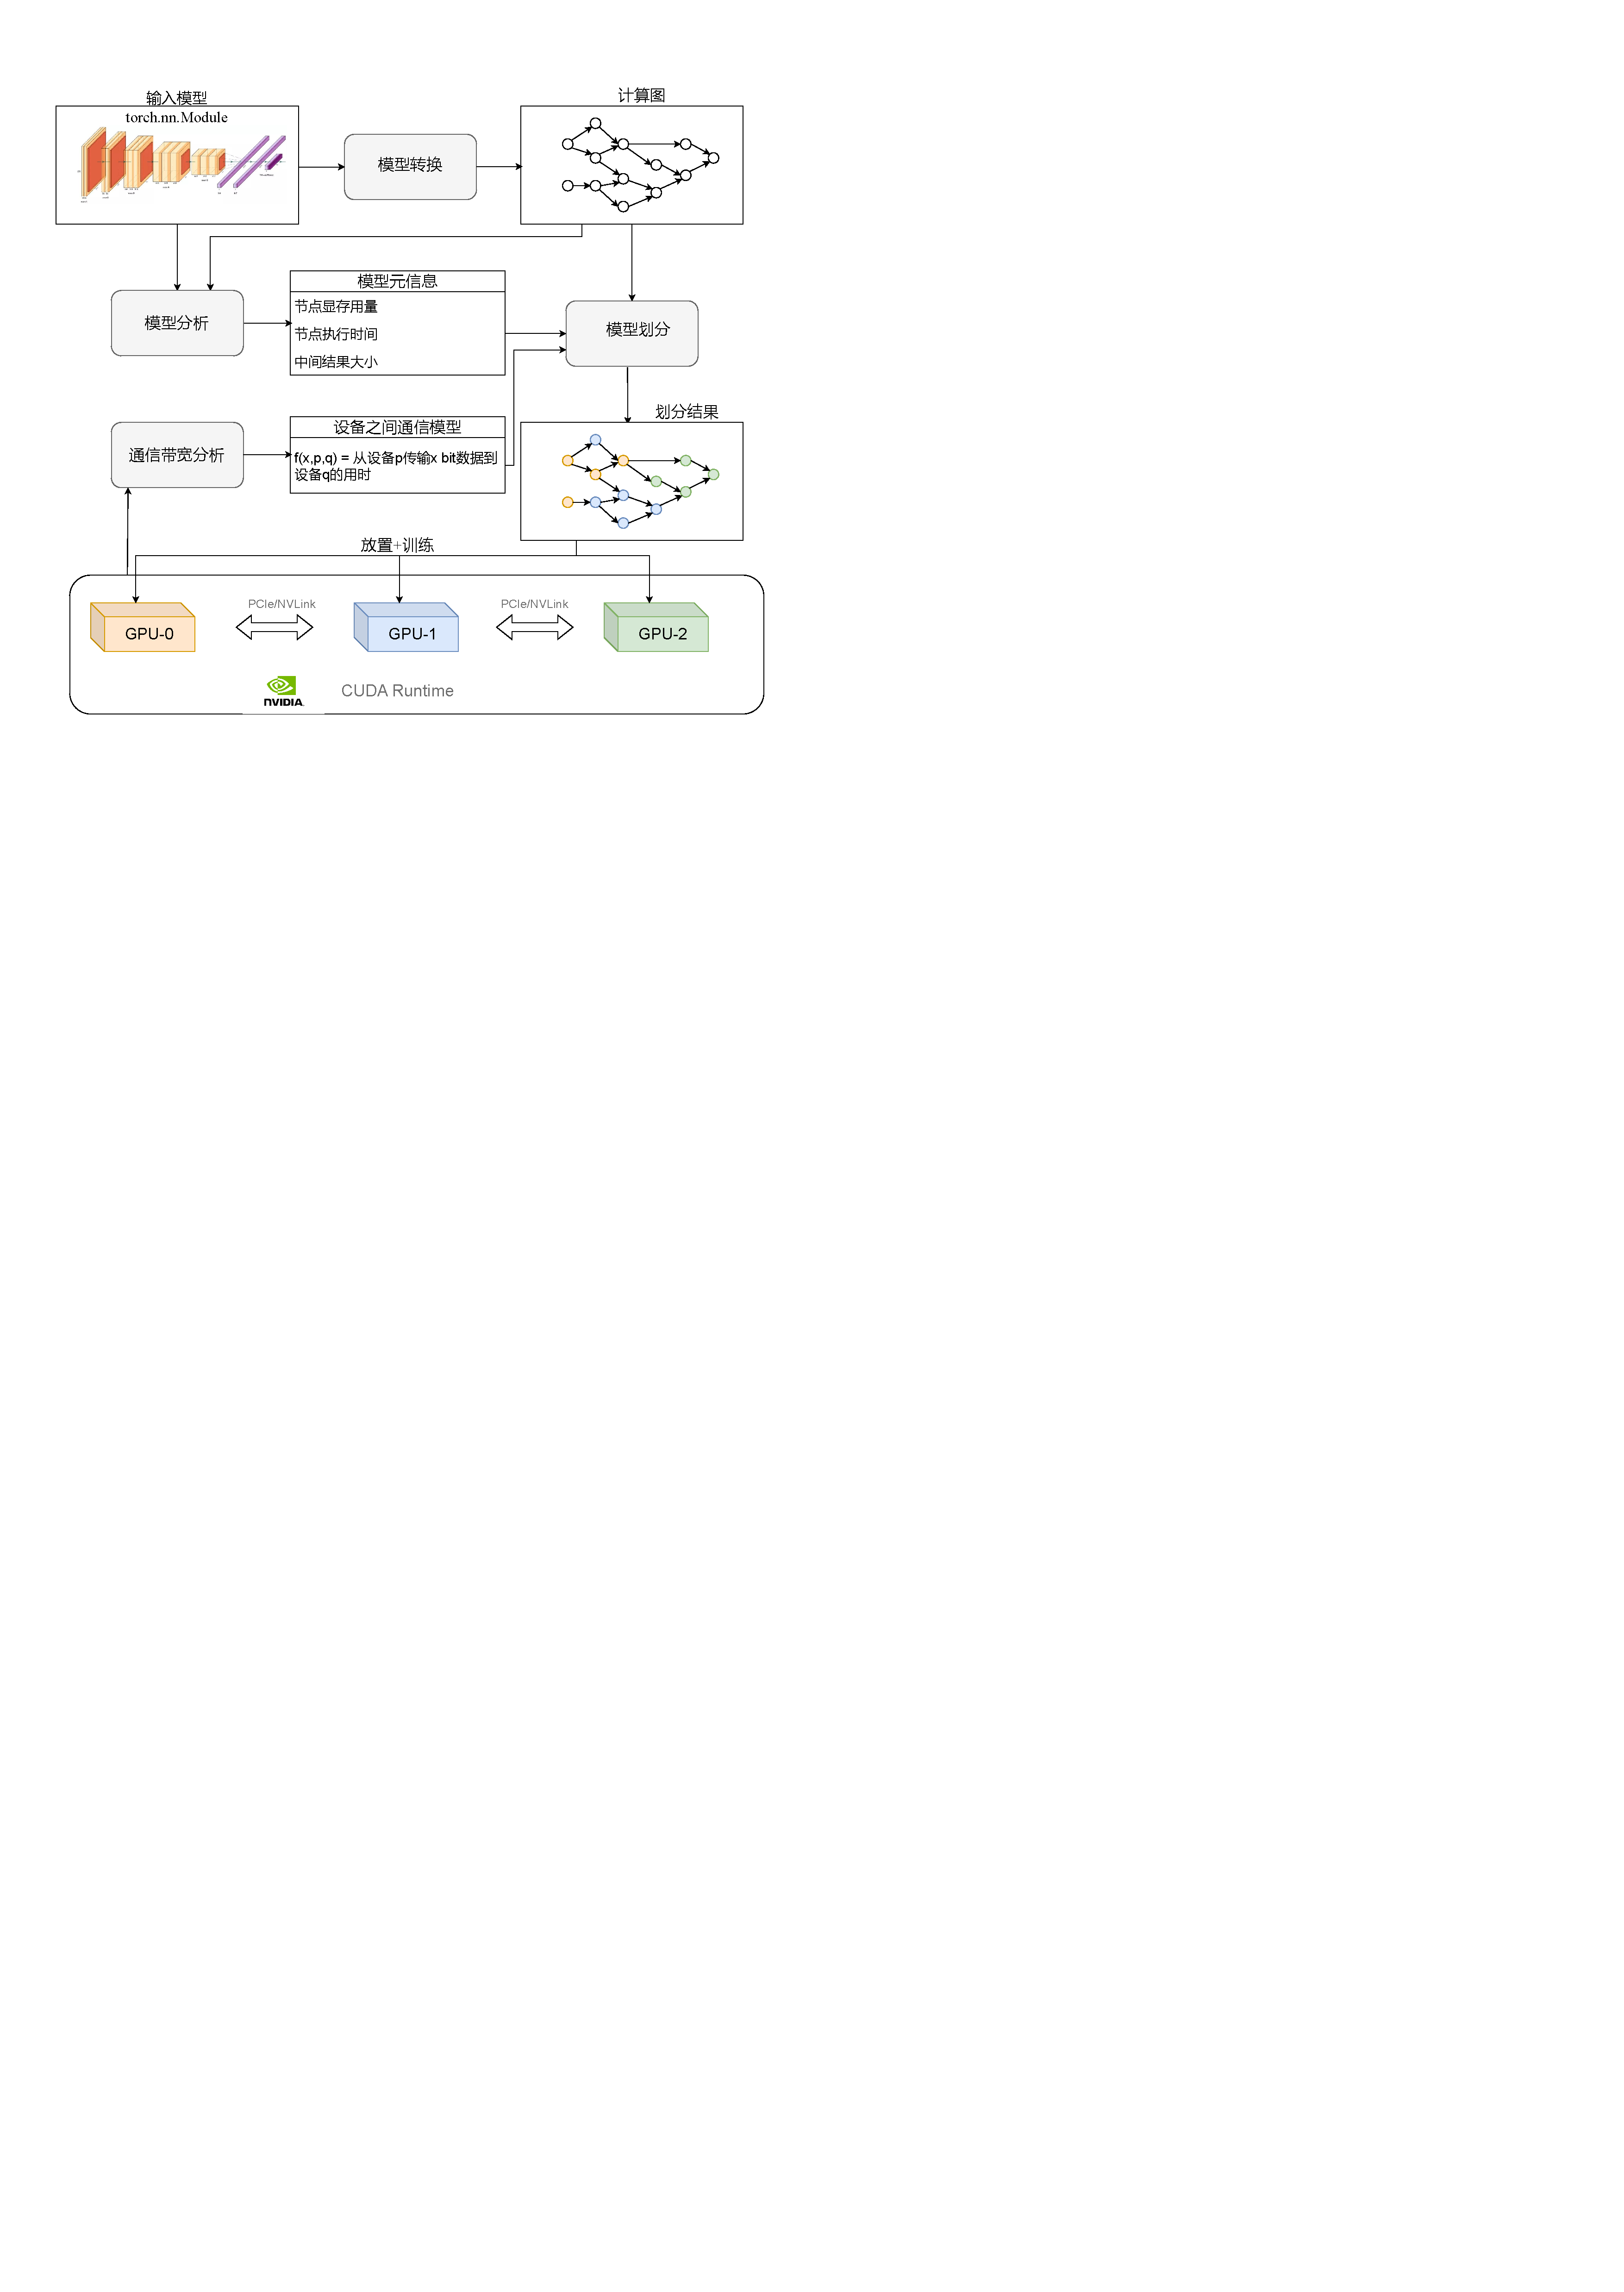
\includegraphics[width=0.95\textwidth]{figure/3-system/arch2.pdf}
	\caption{\sys{} 总体架构}
	\label{fig:arch}
\end{figure}

为了简化大模型的模型并行化训练过程,我们设计了\sys{}。
\sys{} 是基于PyTorch的,针对大型神经网络进行自动化训练的框架。通过提供自动化的模型分析,硬件环境分析,模型转化,模型划分等功能,尽可能简化大模型等训练流程,减少人工参与,解决大模型难以训练的问题。
\sys{} 支持对通用的PyTorch模型进行训练,无需使用者对模型进行预处理。
\sys{}接受用户定义的模型作为输入,并自动完成模型结构理解,对模型进行转换,得到模型底层计算图的中间表示。然后通过动态分析和静态分析的方式,获得模型的元信息,包括计算图中节点的显存用量,计算图中节点的执行时间等。同时,\sys{} 采集参与训练的硬件的信息,并测试设备之间的点对点通信带宽。
然后模型划分模块接受模型元信息、模型计算图以及设备信息为输入,给出模型的划分结果。最后训练模块根据模型的划分结果进行模型到设备的放置,并启动训练流程,完成训练。
整体框架如图 \ref{fig:arch}所示,各个功能模块的简介如下:
\begin{itemize}
	\item \textbf{模型转换模块}: 负责进行模型结构的分析,实现用户输入的PyTorch模型和计算图中间表示的相互转换,从而允许框架对封装层次较高的模型进行进一步细分。
	\item \textbf{模型分析模块}: 通过动态分析和静态分析的方式,获取模型计算图中每个节点的前向传播/反向传播执行用时,计算图中每条边的传输的数据量,计算图中每个节点使用的内存。
	\item \textbf{通信测试模块}: 对参与训练的设备进行通信带宽的基准测试,来获取设备之间的点对点通信带宽,用于估算跨设备的通信时间。
	\item \textbf{模型划分模块}:模型划分模块是\sys{} 的核心模块,该模块根据模型分析模块和通信测试模块的输出,使用约束优化对模型计算图进行划分。
	\item \textbf{训练运行时模块}:划分好的模型由运行时模块放置到设备上进行训练,改模块根据计算图的划分结果重建模型,并处理节点之间的跨设备通信。
\end{itemize}



\section{模型和计算图的转换}
\label{sec:convertion}
% 1: 原始模型 - ONNX -> IR 
% 2: IR - fx.Graph -> 等价模型

\subsection{获取计算图}
在PyTorch中,通常使用继承了\texttt{torch.nn.Module}的类对模型进行描述,模型的计算图由\texttt{forward}函数隐式定义,在运行时由框架动态生成。
为了便于后续对模型进行划分,我们需要提取出隐式定义的计算图,将其转换为某种中间表示,例如由邻接表或者邻接矩阵所表示的图。

\begin{figure}[h]
	\centering
	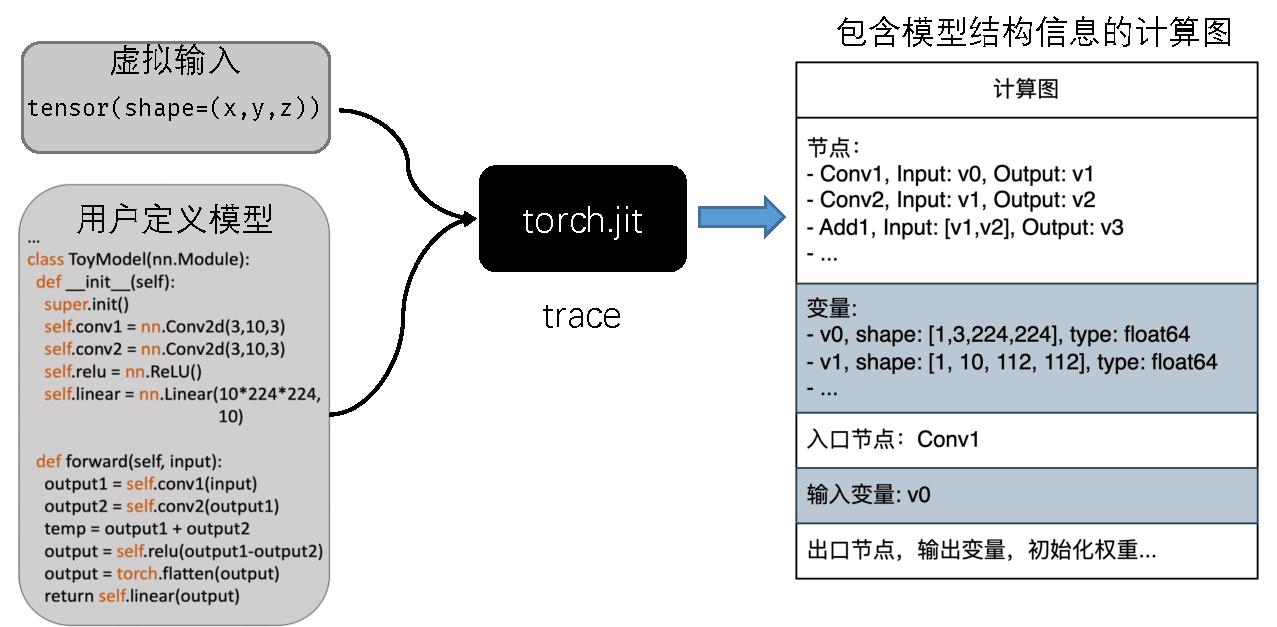
\includegraphics[width=0.9\textwidth]{figure/3-system/2ir.pdf}
	\caption{模型转换为中间表示}
	\label{fig:2IR}
\end{figure}

图 \ref{fig:2IR} 描述了从原始模型定义到中间表示的流程,首先框架将对模型进行即时编译和导出,将原始的PyTorch模型转换为通用的ONNX(Open Neural Network Exchange)格式\footnote[1]{https://github.com/onnx/onnx}的模型文件,然后框架读取模型文件,将其反序列化为计算图的中间表示。
其中,ONNX是一种通用的模型描述的格式。
作为一种较为通用的模型描述格式,ONNX内置了大量算子可以对应到不同框架的算子,表 \ref{table:onnx-operators}展示了部分ONNX算子和对应的PyTorch算子。

\begin{table}
	\centering
	\caption{ONNX与PyTorch的部分算子对应}
	\label{table:onnx-operators}
	\begin{tabularx}{\linewidth}{ p{2cm}  p{2.2cm}  p{5.8cm}  X  }
		\toprule
		\textbf{算子} & \textbf{输入} & \textbf{描述} & \textbf{对应PyTorch} \\
        \midrule
        Transpose & 
        input:tensor; perm:tuple; &
        根据perm对input的维度进行重新排列,功能类似于numpy中的np.permute
        & permute \\
        \midrule
        Flatten & 
        input:tensor; axis:int; &
        对输入张量input进行扁平化操作,输出output为2D矩阵。axis指定输出矩阵第一维的结束维度。
        例如输入张量的形状为$(a,b,c,d)$,axis=2,则输出矩阵的形状为$(ab, cd)$&
        flatten
        \\
        \midrule
        Upsample &
        input:tensor; scale:tensor;&
        对输入张量进行上采样,scale是一个长度等于input维数的张量,每一项指定了input的一个维度进行上采样时的缩放参数。例如对形状为$(a,b,c)$的输入张量进行上采样,scale=$(2,3,4)$,则输出张量的形状为$(2a,3b,4c)。$&
        interpolate
        \\
        \midrule
        Conv &
        input:tensor; w:tensor; bias:tensor; &
        使用w作为卷积核权重对输入张量input进行卷积运算,如果bias非空,则结果加上bias。&
        nn.Conv1d; nn.Conv2d; nn.Conv3d;
        \\
        \bottomrule
	\end{tabularx}
\end{table}

我们首先使用\texttt{torch.onnx.export} 对原始模型进行及时编译,追踪模型在运行过程中所使用的算子,得到等价的ScriptModule,然后将结果导出为ONNX格式的模型。
ONNX中定义了Graph,Node,Variable等结构体,解析ONNX文件,就可以得到模型的计算图的中间表示。
我们使用邻接表的形式描述计算图,在计算图中,如下字段会被存储:
\begin{itemize}
	\item Nodes: 记录计算图中所有的节点,每一项都是一个节点,代表一个算子。对于每个算子,我们记录它的类型,名称,输入变量和输出变量,注意有一些算子例如Add会有超过一个输入变量,因此输入变量和输出变量都使用集合进行存储。
	\item Variables: 记录图中的所有边,每一项都是一个边,代表一个变量。对于每个变量,我们记录它的数据类型,名称以及形状。后续我们可以根据数据类型和形状推断出变量使用的显存大小。
	\item EntryNodes:计算图的入口节点,可能不唯一。
	\item InputVariables: 计算图的输入变量,可能不唯一。
	\item OutputVariables: 计算图的输出变量,可能不唯一。
	\item Initializers: 对于某些特殊的算子,有可能需要为其提供初始权重,例如批归一化(BatchNormalization)层。
\end{itemize}

\subsection{模型重建}
除了从原始模型中提取出模型底层的计算图之外,自动化模型转换模块的另一个重要功能是从计算图中间表示重建出和原模型等价的PyTorch模型。
在原始的模型定义中,计算图的节点和边在\texttt{forward}函数中被隐式定义,这种隐式定义计算图的方式为后续的模型划分和放置带来了困难。
当我们在计算图中应用了模型的划分结果后,需要在计算图中添加额外的通信节点。例如计算图中存在边$\langle u,v\rangle$,节点$u$被划分到了设备-0上,节点$v$被划分到了设备-1上,那么必须在$u$和$v$之间添加额外的通信节点$w$,$w$负责从设备-0上接受变量,并将其放置到设备-1上。
也就是说原来的边$\langle u,v\rangle$会被$\langle u, w\rangle$ 和$\langle w,v\rangle$取代。

由于在原始模型中计算图是隐式定义的,因此上述对于计算图进行修改的操作难以在不修改\texttt{forward}函数本身的条件下实现。
为了更方便的修改计算图,我们的解决方案是从原始计算图中重建出和原模型等价的\texttt{fx.GraphModule}。
\texttt{torch.fx} \upcite{torchfx} 工具包提供了对PyTorch模型进行变换以及构建PyTorch模型的功能。
与通过\texttt{forward}对计算图进行隐式定义的\texttt{nn.Module}实例不同,\texttt{GraphModule}通过直接定义计算图的方式构建模型。
一个\texttt{GraphModule}中包含了若干算子,以及一个用于描述这些算子之间计算依赖关系的\texttt{fx.Graph}实例。
在\texttt{fx.Graph}中,有一系列节点,每个节点除了记录对应的算子,还记录了参与运算的变量,通常参与运算的变量是其他节点的输出。

\begin{lstlisting}[language=Python, caption={模型重建}]
import torch.fx as fx 
torch_graph = fx.Graph() 
place_holders = {}
wrapper_module = nn.Module()
# nodes are already topo-sorted.
for ir_node in graph.nodes:
  node = convert_to_torch(ir_node)
  wrapper_module.add_module(node, name=ir_node.name)
  args = []
  for var in ir_node.inputs:
    if var.type == GRAPH_INPUT:
	  args.append(graph.inputs[var.id])
	elif var.type == GRAPH_INITIALIZER:
      args.append(graph.initializers[var.id])
	elif var.type == NODE_OUTPUT:
	  input_node_name = g.find_node_name(var)
	  input_node = place_holders[input_node_name]
	  args.append(input_node)
  place_holders[ir_node.name] = torch_graph.call_module(ir_node.name, args)
return fx.GraphModule(graph=torch.graph, root=wrapper_module)
\end{lstlisting}

在获取到计算图之后,我们可以根据计算图构建出等价的模型,上面的伪代码展示了构建的过程。
首先创建出记录计算图信息的\texttt{fx.Graph}对象,以及用于存储计算图中节点对应的PyTorch算子的容器\texttt{wrapper\_module}。
然后按照拓扑排序的顺序对计算图中的节点进行遍历,对于每个中间节点\texttt{ir\_node},寻找它的输入变量,如果输入变量来自计算图,则直接使用变量名,如果输入变量来自其他节点的输出,则使用该节点作为输入。
所有输入变量确定后,用\texttt{placer\_holders}记录算子之间的计算关系。
图中所有节点遍历完成后,就得到了存储所有节点对应的PyTorch算子的容器\texttt{wrapper\_module},以及记载了这些算子之间计算关系的\texttt{torch\_graph},从\texttt{wrapper\_module}和\texttt{torch\_graph}就可以得到所需的\texttt{fx.GraphModule},并返回。

\section{通信代价建模}
\label{sec:commu}
% 为什么: 通信不可忽略; 通信链路异构
% 怎么做: 线性建模
分布式深度学习不仅是计算密集型任务,也是通信密集型任务。
在进行模型并行化训练时,模型被分散在不同的设备上,前向传播的中间结果和反向传播的梯度通过设备之间的通信在不同的算子之间传输。
而设备之间的通信时间不可忽略,图 \ref{fig:overhead} 展示了使用4张1080Ti GPU在CIFAR-10 \upcite{cifar} 数据集上训练VGG19 \upcite{vgg} 模型时,不同的步骤耗时的分解。
可以发现即使CIFAR-10是很小的数据集,通信时间也占据了总用时的40\%。

\begin{figure}[h]
	\centering
	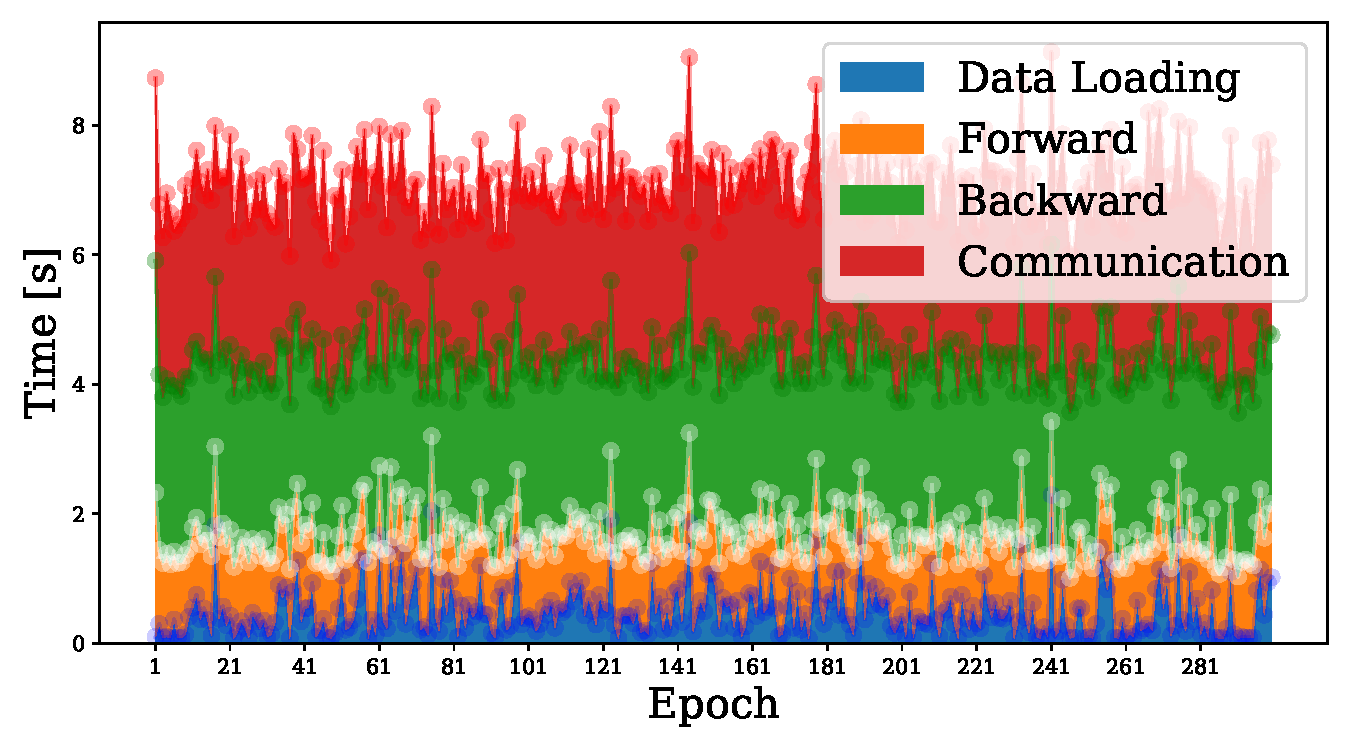
\includegraphics[width=0.85\textwidth]{figure/3-system/overhead_decomposition.pdf}
	\caption{训练用时分解}
	\label{fig:overhead}
\end{figure}

\begin{figure}[h]
	\centering
	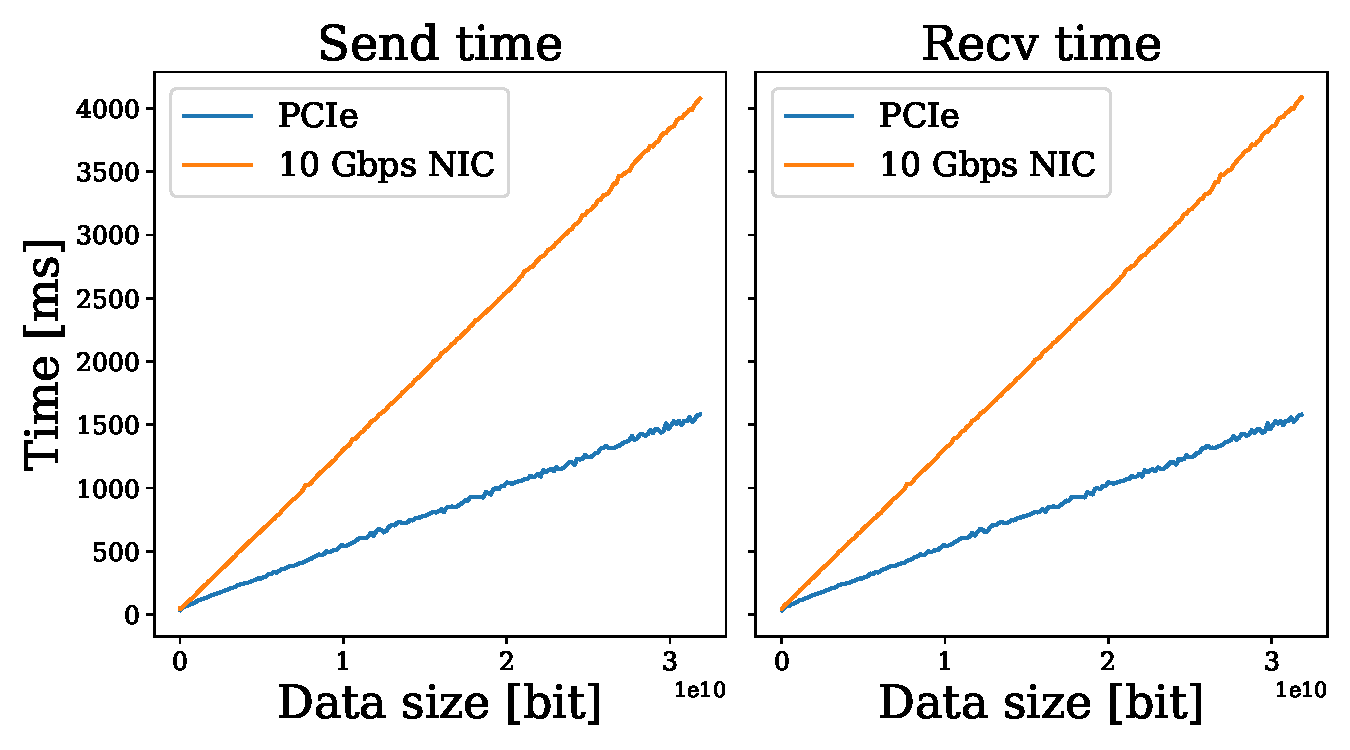
\includegraphics[width=0.85\textwidth]{figure/3-system/commu.pdf}
	\caption{通信用时和传输数据量的关系}
	\label{fig:linear}
\end{figure}
在神经网络模型中,节点与节点之间通信的数据量会随着节点类型变化而变化。
例如某个节点对应卷积操作时,输出数据的通道数目相比于输入数据会增加,因此输出数据的大小会增加,所需要的通信时间也更多。
而某个节点如果对应池化操作,输出数据可以看作是对输入数据进行下采样,因此输出数据的大小会减少,所需要的通信时间也更少。
因此在对模型进行划分时,我们需要考虑节点的输出数据的大小,通过合理的划分,让设备与设备之间传输的数据量更少,从而达到优化通信代价的效果。

另一方面,在优化通信代价时,除了需要考虑节点之间通信的数据量,也需要考虑设备与设备之间的通信链路。
在计算集群中,设备之间的通信链路往往是异构的。
例如设备可以通过高性能专用通信设备,如NVLink,NV-Switch通信,也可能通过通用的PCIe或者以太网进行通信。
因此在进行通信代价优化时,设备之间通信链路的异构性也需要被考虑。
我们设计了通信测试模块来对设备之间的点对点通信带宽进行建模。
图 \ref{fig:linear}展示了设备通过10Gbps的以太网卡和通过PCIe Switch进行通信时,传输的数据量和用时的关系,可以发现传输数据量和通信时间呈现出线性关系,因此我们使用线性模型对通信代价进行建模。
通信测试模块在设备之间发送不同大小的数据包,并记录数据包对应的传输时间,
然后对传输时间和数据大小两类数据进行线性拟合,获得通信时间的预测模型,在给定数据包大小的情况下,可以准确预测通信时间。
通信时间预测模型在后续的模型划分模块中用来预测给定的划分的通信代价,指导模型划分模块对通信代价进行优化。

\section{显存代价估计}
\label{sec:mem}
% 1. 模型: 参数 + 梯度 + 动量
% 2. 中间结果: 张量大小 + 梯度 + 动量 
模型并行化主要解决单个设备的显存容量有限,难以满足大模型训练时对于显存的需求。
设备的显存容量可以通过查看设备信息获得,而模型训练时所需要的显存对于开发者来说是未知的,当开发者进行手动模型划分时,难以保证划分后的模型在设备上训练时仍然满足设备的显存限制,因此我们需要一种可以预估模型显存占用的方法,用来判断某种模型划分是否可以满足当前硬件设备的限制。

\begin{table}
	\centering
	\caption{计算图的显存开销}
	\label{table:model-mem}
    \begin{tabularx}{\linewidth}{p{2.4cm} p{2.6cm} X }
        \toprule
        \textbf{种类} & \textbf{类型} & \textbf{描述} \\
        \midrule
        \multirow{2}*{节点} & 参数 & 算子中可以学习的参数,例如卷积中的卷积核 \\
        \cmidrule{2-3}
        & 参数梯度 & 在反向传播过程中计算出的用于更新参数的梯度,大小与对应参数大小相同,随着优化器的不同,可能还有动量与二阶动量 \\
        \midrule
        \multirow{4}*{边} & 模型输入 & 计算图的入口节点从数据加载器获得的输入数据批(data batch) \\
        \cmidrule{2-3}
        & 算子输入 & 计算图中算子的输入变量 \\
        \cmidrule{2-3}
        & 算子输出 & 计算图中算子的输出变量,对于该算子的后继算子来说,如果后继和该算子在同一个设备上,则该算子的输出变量等同于后继算子的输入变量 \\
        \cmidrule{2-3}
        & 变量梯度 & 在反向传播过程中计算出的变量梯度,用于计算参数梯度 \\
        \midrule
        固定开销 & CUDA上下文 & 包括CUDA运行时,cuDNN Lib加载等需要占用的显存 \\
        \bottomrule
    \end{tabularx}
\end{table}

由于我们在计算图的层面对模型进行划分,因此显存预估也在计算图的层面上进行。
计算图中,每个节点所对应的算子会消耗显存,每个边也会消耗显存,具体来说,我们可以将模型的显存占用分为以下的三部分:
\begin{itemize}
	\item 模型参数:模型参数也就是模型中需要进行学习和更新的张量,这部分显存消耗来自于计算图中的节点,每个节点对应的算子如果有需要进行学习的参数,都会占用一部分显存来存储这些参数。
	\item 中间结果:在计算图中,每个节点代表一个算子,而每条有向边就对应算子运算的结果。
	这些中间结果由前一个算子输出,并且作为后一个算子的输入。中间结果会被暂存,用来在反向传播时计算梯度。
	\item 梯度:在反向传播过程中,被计算得到用于更新模型参数。一般来说梯度所使用的显存大小等同于模型参数所使用的显存大小,对于某些优化器来说,除了需要计算梯度,还会存储动量(Momentum)以及二阶动量,因此会有额外的显存开销。
	总显存开销应该是模型参数所需的显存开销的整数倍。
\end{itemize}

表 \ref{table:model-mem} 详细的描述了模型训练中的几种显存开销,下面我们将介绍如何对这几种显存开销进行预估。
\begin{table}
	\centering
	\caption{几种算子模型参数显存开销}
	\label{table:operator-mem}
    \begin{tabularx}{\linewidth}{ p{2.4cm} p{3.8cm} X }
        \toprule
        \textbf{算子} & \textbf{参数大小} & \textbf{描述} \\
        \midrule
        Conv2D & $C_{in} \times C_{out} \times K_{h} \times K_{w}$ & 二维卷积算子的模型参数量等于卷积核的数目乘以每个卷积核的大小 \\
        \midrule
        Linear  & $F_{in} \times F_{out} + F_{out}$ & 线性变换算子的模型参数量等于线性变换矩阵大小加上偏置大小 \\
        \midrule
        BatchNorm2D & $2\times C $ & BatchNorm2D对输入执行批归一化,也就是计算$y=\frac{x-E(x)}{\sqrt{var(x)+\epsilon}} \times \gamma + \beta$,对于输入数据的每个通道,都需要存储相应的$\gamma$和$\beta$ \\
        \bottomrule
    \end{tabularx}
\end{table}

\begin{algorithm}[h]
	\caption{判定划分是否满足内存约束}
	\label{alg:estimate-mem}
	\begin{algorithmic}[1]
	\REQUIRE $\mathit{NodeToDevice}$, $\mathit{Nodes}$, $\mathit{MemCapacity}$
	\ENSURE  $\mathit{isValid}$
	\STATE   $\mathit{VariablesOn} \leftarrow \mathrm{Map}[\mathrm{int}, \mathrm{Set}]$
	\STATE   $\mathit{DeviceMem}_{0,1,\dots,n} \leftarrow 0$
	\FOR{ $\mathit{Node}\ n\ \in \mathit{Nodes}$ }
		\STATE $device \leftarrow \mathit{NodeToDevice}[n]$
		\FOR{$\mathit{Variable}\ input\ \in\ n.\mathit{inputs}$}
			\IF{$input \not\in \mathit{VariablesOn}[device]$}
				\STATE $\mathit{VariablesOn}[device].add(input)$
				\STATE $\mathit{DeviceMem}_{device}\ \leftarrow \ \mathit{DeviceMem}_{device} + input.size \times 2 $
			\ENDIF
		\ENDFOR
		\FOR{$\mathit{Variable}\ output\ \in\ n.\mathit{outputs}$}
			\IF{$output \not\in \mathit{VariablesOn}[device]$}
				\STATE $\mathit{VariablesOn}[device].add(output)$
				\STATE $\mathit{DeviceMem}_{device} \leftarrow  \mathit{DeviceMem}_{device} + output.size \times 2 $
			\ENDIF
		\ENDFOR
		\STATE $\mathit{DeviceMem}_{device} \leftarrow  \mathit{DeviceMem}_{device} + n.weight.size + n.gradient.size$
	\ENDFOR
	\STATE $\mathit{isValid}\leftarrow \mathrm{TRUE}$
	\FOR{$i:=0; i < n; i++$}
		\IF{$\mathit{DeviceMem}_{i} > \mathit{MemCapacity}_{i}$}
			\STATE $\mathit{isValid}\leftarrow \mathrm{FALSE}$
		\ENDIF
	\ENDFOR
	\RETURN $\mathit{isValid}$
	\end{algorithmic}
\end{algorithm}

\textbf{计算图节点开销}: 计算图节点的显存开销来自模型参数和训练过程中用于优化模型参数所产生的梯度以及可能的动量,二阶动量等。大部分节点所对应的算子,例如激活函数算子,二元运算算子等都没有可以学习的参数,因此这些算子的节点不会直接产生显存开销。表 \ref{table:operator-mem} 列举了部分会产生模型参数显存开销的算子,以及对应的开销的计算方法。
模型参数梯度与模型参数大小相同,因此显存开销相同。但是不同的优化器中,除了需要使用梯度,也会使用动量或者二阶动量来记录梯度下降的历史信息,控制梯度下降的优化方向。例如在Adam优化器 \upcite{adam} 中,会用到动量和二阶动量,因此会产生为模型参数显存开销3倍的显存开销,用于存储梯度、动量和二阶动量。

\textbf{计算图边开销}: 计算图中,每个边都代表一个中间结果变量,存储这些变量和变量的梯度会带来显存开销。此外,如果边两端的节点在同一个设备上,那么边上的变量只会产生一次开销,而如果边两端的节点在不同的设备上,则边上的变量会分别作为节点输入和节点输出在两个设备上都产生显存开销。

\textbf{固定显存开销}: 固定显存开销主要来自加载模型训练所需的算法库,这部分开销相对固定,可以在启动任务前通过API得到。

在得到计算图中每个节点和每条边的显存开销后,我们就可以将其作为模型的元信息输入到模型划分模块中,来指导模型划分模块进行模型划分,避免划分后的模型过大,导致某个设备出现显存溢出的问题。
算法 \ref{alg:estimate-mem}展示了如何判定给定的模型划分是否可以满足内存约束。
算法的输入中,$\mathit{NodeToDevice}$ 是划分结果,是一个从节点到设备的映射。
$\mathit{Nodes}$ 是计算图中所有节点按照拓扑排序后得到的节点列表,列表中的每一项都是一个节点,记载了节点的输入变量,输出变量,每个变量的大小,以及节点的参数大小。
$\mathit{MemCapacity}$ 是设备的显存容量。
首先,算法中声明了临时变量$\mathit{VairablesOn}$,用来存储某个设备上已经存在的变量。
算法的最外层循环对节点列表进行遍历,对于每个节点,分别遍历它的输入变量,输出变量,如果变量不在节点所在的设备上,则将变量加入到当前设备上,并将变量使用的显存加到当前设备的显存用量$\mathit{DeviceMem}$中。
最后将节点的参数,梯度,动量的显存占用也加入到节点所在的设备上,判定设备上的显存申请是否大于设备的显存容量,并返回结果$\mathit{isValid}$。



\section{计算代价分析}
\label{sec:time}
% HOOK + Virtual Node for Edge + 代码展示
获取一个好的模型划分的前提是模型划分模块有足够的模型元信息来指导模型的划分,除了需要模型计算图中每个节点的显存用量,还需要每个计算节点的计算用时。
有了每个节点计算用时,就可以指导模型划分生成训练用时更短的划分方案。
因此我们设计了计算代价分析模块,用于获取计算图中每个节点在训练时的前向传播用时和反向传播用时。
为了便于表述,我们记$FP_{v}$表示节点$v$的前向传播用时,$BP_{v}$表示节点$v$的反向传播用时。

由于计算用时和多种因素有关,包括使用的CUDA版本,硬件性能,具体的算子底层实现等,因此我们难以通过静态的方式确定每个算子的用时,所以我们采用动态分析的方式对每个算子的计算用时进行采集。
\sys{}基于PyTorch实现,PyTorch提供了Hook机制,帮助开发者注册模型训练时关键事件的回调(Call Back)函数,比如某个算子前向传播开始的事件。下面是PyTorch中支持的4种回调函数的注册方法:
\begin{itemize}
	\item \texttt{torch.Tensor.register\_hook(func)}: 向某个张量注册回调函数,当和该张量相关的梯度被计算出时,回调函数被触发。回调函数接受旧的梯度作为输入,可以在回调函数中对梯度进行修改操作,返回修改后的梯度。常用于在张量进行更新前,对梯度进行修改。
	\item \texttt{torch.nn.Module.register\_forward\_pre\_hook(func)}: 向某个神经网络模块注册回调函数,该回调函数在模块执行\texttt{forward()}方法前被调用,回调函数接受前向传播的输入,返回修改后的输入。常用于在模块执行前向传播之前,对输入进行修改。
	\item \texttt{torch.nn.Module.register\_forward\_hook(func)}: 向某个神经网络模块注册回调函数,回调函数在模块执行\texttt{forward()}方法后被调用,用来获取和修改前向传播的输出。
	\item \texttt{torch.nn.Module.register\_backward\_hook(func)}: 向某个神经网络模块注册回调函数,在该模块完成反向传播计算出梯度后被调用,可以用来获取并修改梯度。
\end{itemize}

通过PyTorch的Hook机制,可以获取模型计算图中各个节点在训练过程中的关键事件,比如前向传播开始,前向传播结束等,记录这些关键事件发生的时刻,就可以计算得到每个节点前向传播和反向传播计算过程的用时。
需要注意的是,PyTorch并没有提供记录某个模块反向传播事件开始的事件的方法,因此我们需要对原有模型进行修改。

我们设计了\texttt{WrapModule}类,该类继承自\texttt{torch.nn.Module}。
该类中封装了一个计算图中的节点,而且可以根据需要,动态为该节点添加虚拟后继节点,通过捕捉虚拟后继节点的反向传播完成事件,就可以得到原始节点的反向传播开始事件,从而计算出原始节点的反向传播用时,以下的代码展示了\texttt{WrapModule}的实现。
如代码所示,当调用\texttt{profile}方法时,通过设置\texttt{enable}可以开启计算时间记录或者关闭计算时间记录,当计算时间记录开启时,会为\texttt{self.\_torch\_module}添加虚拟后继节点,计算时间记录关闭时,则会移除该虚拟后继节点。

\begin{lstlisting}[language=Python, caption={WrapModule实现}]	
class VirtualModule(nn.Module):
	def forward(self, x, *args):
		return (x, ) + args if args else x
class WrapModule(nn.Module):
	def __init__(self, torch_module: nn.Module, node_name: str):
		super().__init__()
		self._torch_module = torch_module
		self._wrapped_module = torch_module
		self._virtual_successor = VirtualModule()

	def forward(self, *args, **kwargs):
		return self._wrapped_module(*args, **kwargs)
	
	def profile(self, enable:bool=True):
		if enable:
			# 开启计算时间记录
			self._wrapped_module = Sequential(self._torch_module, self.virtual_sucessir)
			...
		else:
			# 关闭计算时间记录
			self._wrapped_module = self._torch_module
			...
\end{lstlisting}

\begin{figure}[h]
	\centering
	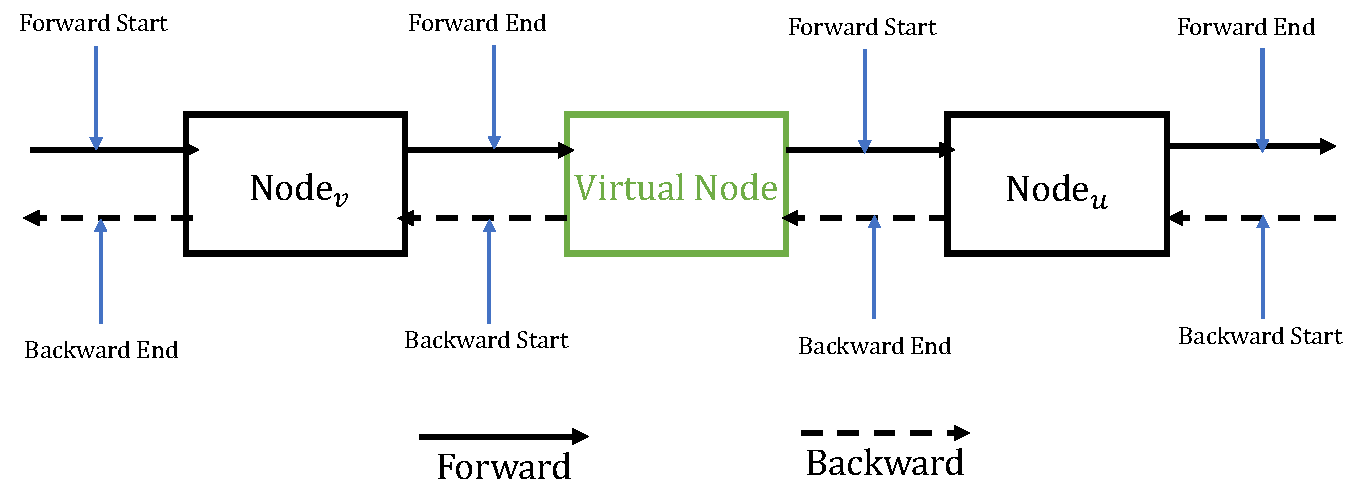
\includegraphics[width=0.8\textwidth]{figure/3-system/profile.pdf}
	\caption{计算代价分析}
	\label{fig:profile}
\end{figure}

在计算时间记录开启时,除了添加虚拟后继节点之外,还会注册回调函数函数,我们会记录节点的前向传播开始,前向传播结束,反向传播结束和虚拟后继节点的反向传播开始这四个事件的发生的时间,并计算得到节点的前向传播用时和反向传播用时,图 \ref{fig:profile} 展示了这一过程。
在实际实现中,我们首先使用Beachi \upcite{baechi}中的m-TOPO(带有内存约束的拓扑排序)划分方法对模型进行划分,这种划分方法具有内存约束,而且运行速度快,因此我们选择这种方法。
然后我们将初步划分好的模型放置到设备上,开启计算时间记录,并使用小批量数据进行训练,多次记录每个节点的前向传播和反向传播用时,并通过取平均值的方式减小误差,最后得到每个节点在当前硬件环境下的前向传播和反向传播用时。

\section{模型划分与训练}
\label{sec:partition-and-train}
% 输入, 输出
% Partitioner和Placer的设计
% 训练
在进行完通信代价建模,显存代价估计和计算代价分析三个步骤后,模型划分模块接受模型计算图以及上述三个步骤到输出,进行模型划分以及后续的模型训练。
\begin{figure}[h]
	\centering
	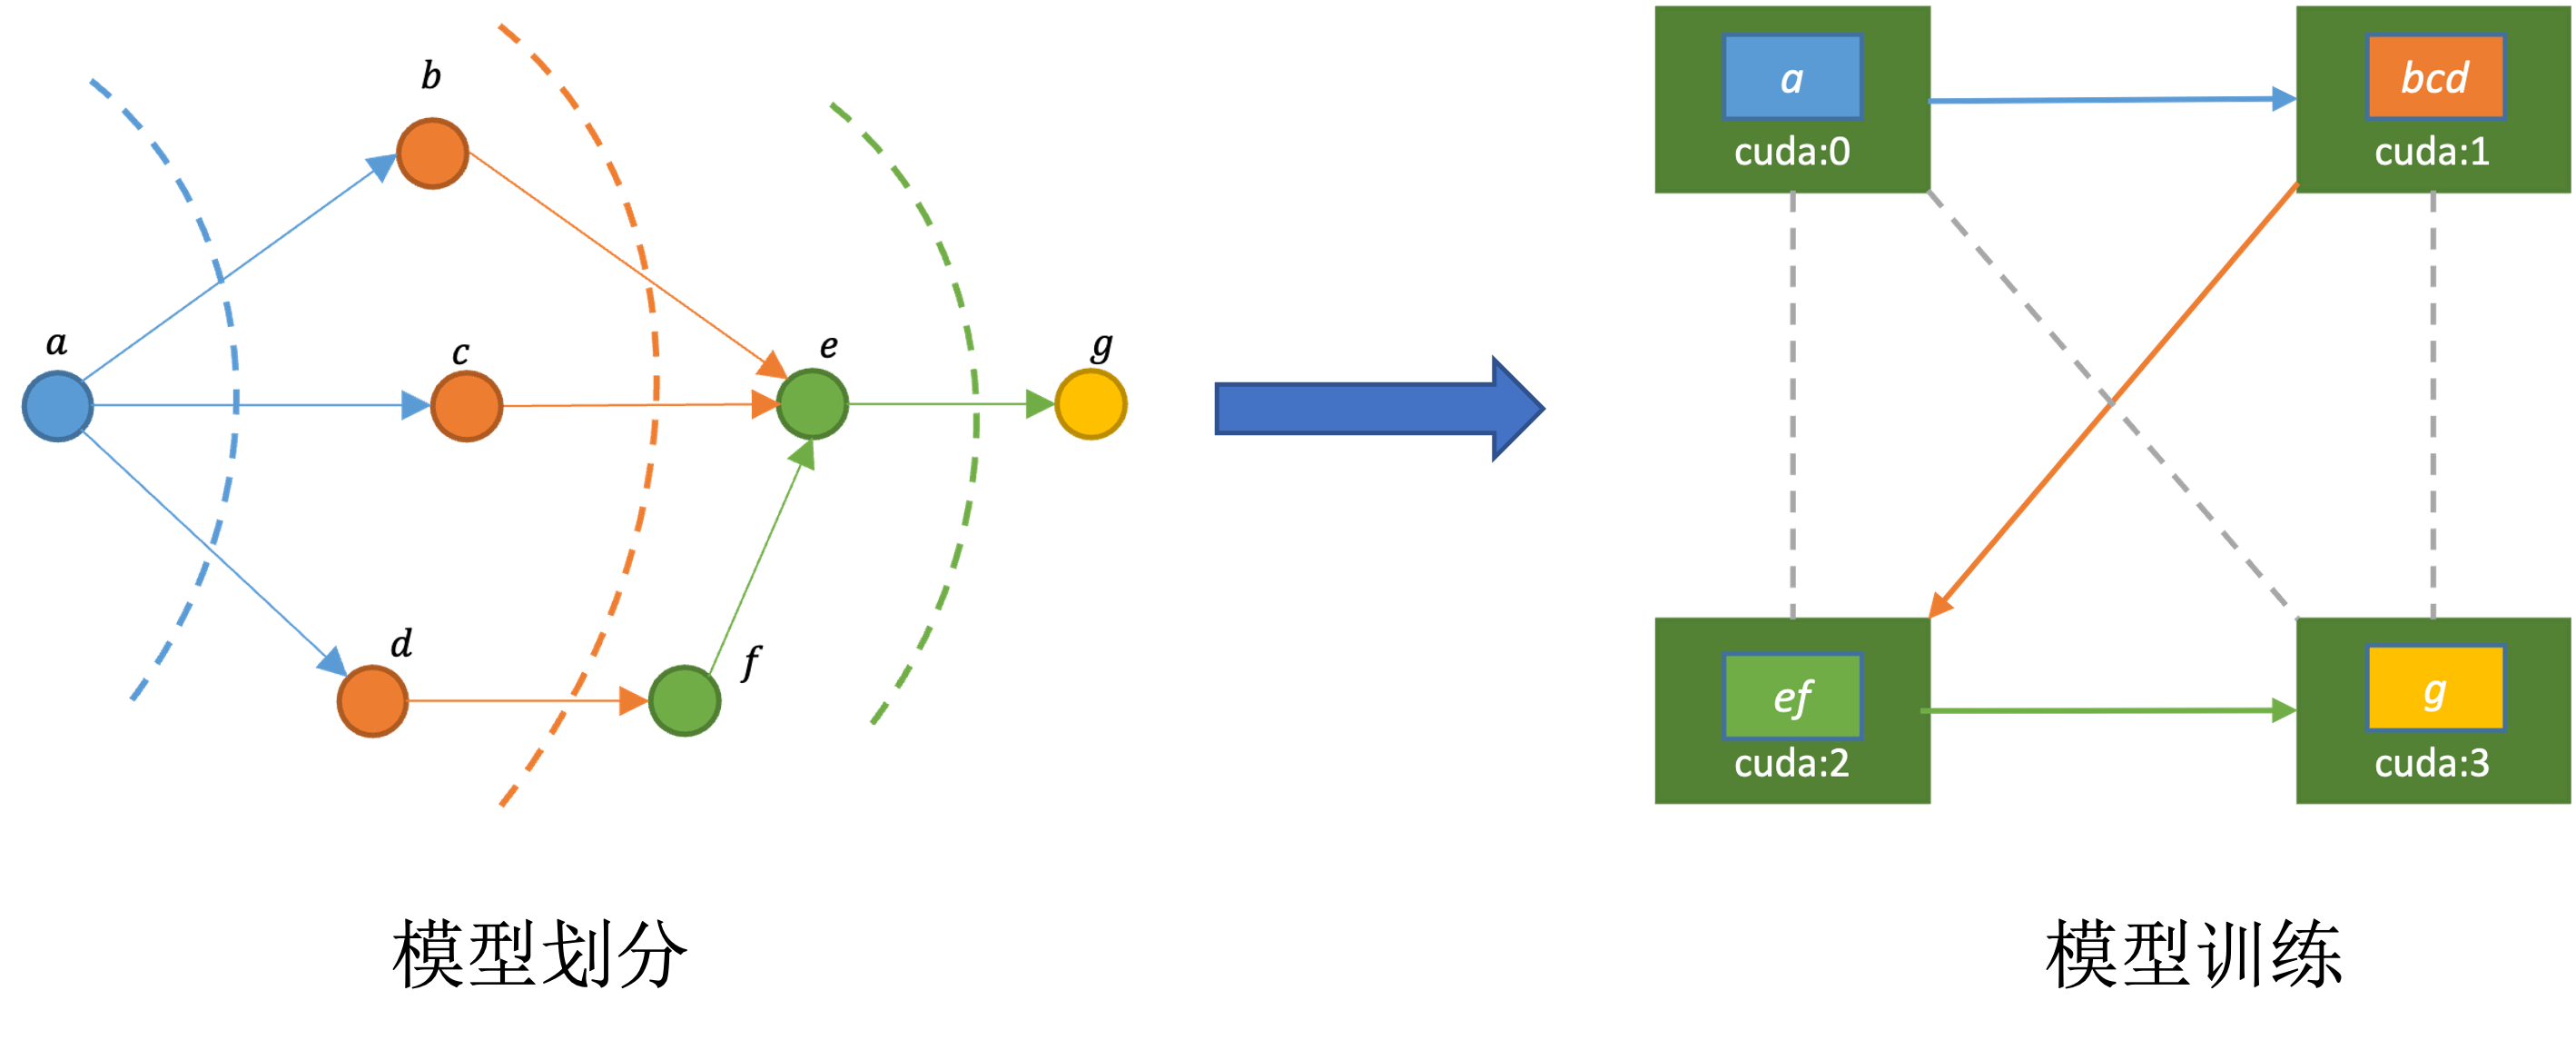
\includegraphics[width=0.9\textwidth]{./figure/3-system/partition_train.png}
	\caption{模型划分与训练}
	\label{fig:partition-and-train}
\end{figure}

图 \ref{fig:partition-and-train} 展示了模型的划分和训练。
模型划分模块为计算图中的节点寻找到设备的映射,在进行划分时,需要考虑设备内存约束,设备之间的通信带宽以及每个节点的计算代价,以最优化训练效率进行划分。
模型划分结束后,我们得到了划分结果,也就是节点到设备的映射。
然后模型训练模块会根据划分结果将模型放置到设备上,并启动训练流程。

在后续的实验中,我们会对比多种模型划分方法的效果,因此我们设计了\texttt{Partitioner}类作为所有模型划分方法的抽象基类。
\texttt{Partitioner}中只有一个\texttt{partition}一个方法,它的输入包括模型的计算图表示,设备信息,每个节点的计算用时信息,每个节点的显存使用信息以及设备之间的通信带宽。
获取输入信息后,\texttt{partition}运行特定的划分算法,给出划分结果,也就是节点到设备的映射。
不同的模型划分方法都需要继承自\texttt{Partitioner}类,并且实现\texttt{partition}方法。
具体划分算法的实现我们将在下一章进行介绍。

\begin{figure}[!h]
	\centering
	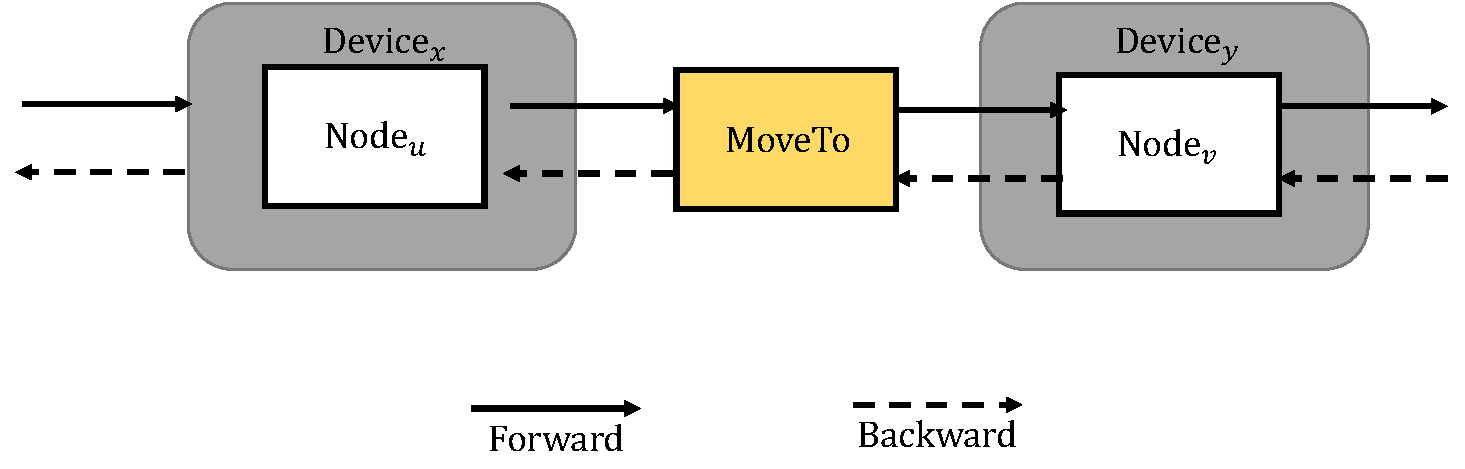
\includegraphics[width=0.9\textwidth]{./figure/3-system/moveTo.pdf}
	\caption{跨设备变量转移}
	\label{fig:move}
\end{figure}

\begin{algorithm}[!h]
	\caption{添加变量转移节点}
	\label{alg:add-move}
	\begin{algorithmic}[1]
	\REQUIRE $\mathit{NodeToDevice}$, $\mathit{Nodes}$, $\mathit{Edges}$
	\ENSURE $\mathit{NewNodes}, \mathit{NewEdges}$
	\STATE  $\mathit{NewNodes} \leftarrow \mathrm{Set}[\mathit{Node}]$
	\STATE  $\mathit{NewEdges} \leftarrow \mathrm{Set}[\mathit{Edge}]$
	\STATE  $\mathit{CriticalEdges} \ leftarrow \mathrm{Set}[\mathit{Edge}]$
	\FOR{$\mathit{Edge}\ e \in \mathit{Edges}$}
		\STATE $\mathit{device}_u \leftarrow \mathit{NodeToDevice}[e.u]$
		\STATE $\mathit{device}_v \leftarrow \mathit{NodeToDevice}[e.v]$
		\IF{$\mathit{device}_u \neq \mathit{device}_v$}
			\STATE $\mathit{CriticalEdges}.add(e)$
		\ENDIF
	\ENDFOR
	\FOR{$\mathit{Edge}\ e \in \mathit{Edges}$}
		\IF{$e \in \mathit{CriticalEdges}$}
			\STATE $w \leftarrow \mathrm{NewMoveNode}(\mathrm{from}:\mathit{device}_u, \mathrm{to}:\mathit{device}_v)$
			\STATE $\mathit{NewEdges}.add(\left\langle e.u,w\right\rangle)$
			\STATE $\mathit{NewEdges}.add(\left\langle w,e.v\right\rangle)$
			\STATE $\mathit{NewNodes}.add(e.u,e.v,w)$
		\ELSE
			\STATE $\mathit{NewEdges}.add(e)$
			\STATE $\mathit{NewNodes}.add(e.u, e.v)$
		\ENDIF
	\ENDFOR
	\RETURN $\mathit{NewNodes}, \mathit{NewEdges}$
	\end{algorithmic}
\end{algorithm}

当得到划分结果后,我们还需要根据划分结果对模型再一次进行修改,显式的为跨设备的边添加变量转移节点。
如图 \ref{fig:move} 所示,计算图中有边$\langle u,v\rangle$,节点$u$被划分到了设备$x$上,节点$v$被划分到了设备$y$上,那么节点$u$的输出变量$u_{out}$默认会被放置在设备$x$上,
当节点$v$尝试去直接读取$u_{out}$时,会触发DeviceMismatch的错误,因此我们需要显式的在$\langle u,v\rangle$上添加将$u_{out}$放置到设备$y$上的变量转移节点。
变量转移节点本身不会带来新的计算代价,可以将变量转移节点看作是通信代价的一种表示,变量转移的过程实际上就是通信的过程。
变量转移节点也是通过继承PyTorch中的\texttt{nn.Module}类实现,在\texttt{forward}函数中,将输入变量放置到指定设备上并传递给后继计算节点去使用。

算法 \ref{alg:add-move} 展示了在计算图中添加变量转移节点的过程。首先我们在计算图中对边进行遍历,寻找所有两端点$u,v$不在相同设备上的边。
对于这种跨越不同设备的边,进行变量转移节点$w$的添加。
变量转移节点$w$会被添加到新的节点集合中,新生成的两条边$\left\langle u,w\right\rangle$ 和 $\left\langle w,v\right\rangle $也会被添加到新的边集。
最后返回新的节点集合和边集,由模型转换模块根据计算图重建模型,进行训练。



\section{本章小结}
本章介绍了\sys{}的设计和每个模块的具体功能。
对于如何实现模型和中间表示之间的相互转换,\sys{}提供了模型转换模块,可以完成用户定义的高层模型和计算图之间的相互转换。
对于模型分析,\sys{}提供了显存代价估计方法和计算代价分析方法,能够得到计算图中节点的显存占用和计算时间,指导模型的划分。
针对计算集群中存在的通信链路的异构性,我们设计了通信代价建模模块,可以对设备之间点对点通信链路进行带宽测试,从而建模通信代价。
获取节点显存占用,节点计算时间和设备通信建模后,\sys{}中的模型划分模块会进行设备划分,模型被划分到多个设备上进行训练。

本章主要介绍\sys{}中功能模块的设计与实现,下一章讲详细介绍模型划分模块中的算法的设计与实现。